% meta.concepts: 3D force equilibrium
% meta.tags: realistic
% acknowledge: Peter Seiler & Luke Melander graciously shared Spring 2019 course material
% source: 2019 P. Seiler AEM2011 HW 2

A wind turbine is installed at the University of Minnesota Eolos Wind Research Field Station. The field station also has a $130 m$ ($426 ft$) tall meteorological tower with sensors for research purposes. The met tower is supported by cables. For simplicity, assume that the tower has three cables attached to the pin at A and anchored on the ground at points B, C, and D. The locations of the various points are given by:
\begin{itemize}
  \item $\bar{A} = 130m \textbf{k}$
  \item $B = 60m \textbf{i} - 40m \textbf{j}$
  \item $C = 60m \textbf{i} + 40m \textbf{j}$
  \item $D = - 40m \textbf{i} + 30m \textbf{j}$
\end{itemize}  
Determine the tension in each cable if the met tower exerts an upward vertical force of $4000 N$ on the pin at $A$.

Reflect on the tensions computed.  What does this say about the supports provided by the assumed cable structure?

\begin{figure}[ht!]
  \centering
  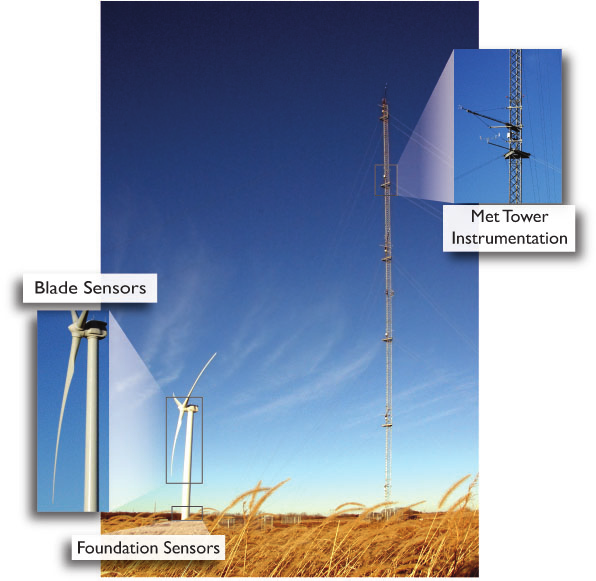
\includegraphics[height=1.8in]{figa.png}
  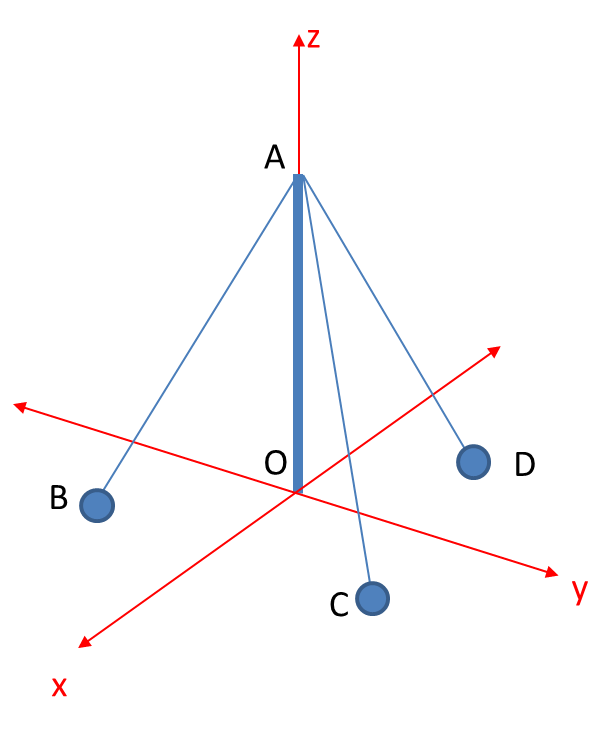
\includegraphics[height=1.8in]{figb.png}
  \caption*{Left: Eolos Field Station (Image courtesy of \texttt{eolos.umn.edu}), Right: Simplified diagram}
\end{figure}

\iftoggle{flagSoln}{%
\vspace{.5cm}
\rule{\textwidth}{.4pt}
\vspace{.5cm}
\textbf{Solution:}
\begin{figure}[ht!]
  \centering
  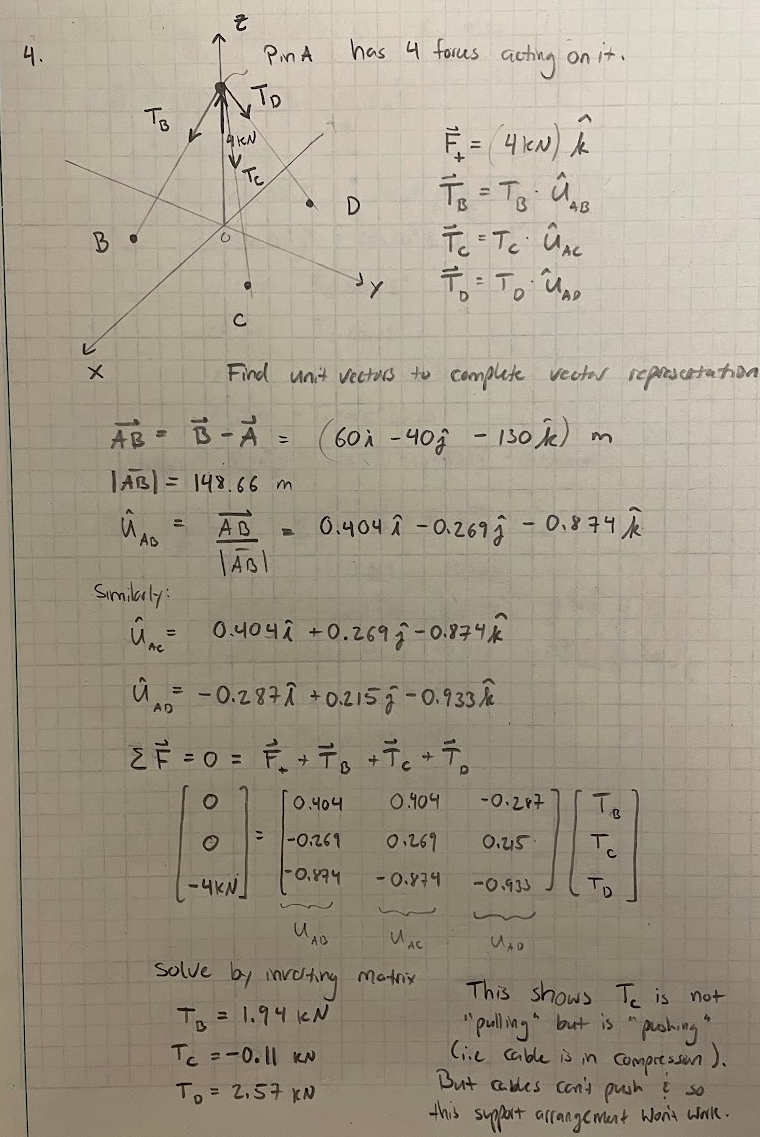
\includegraphics[width=0.9\textwidth,
	           height=0.3\textheight,
		   keepaspectratio]{soln.png}
\end{figure}
}{%
}%
